\documentclass[../../main.tex]{subfiles}
\begin{document}

{\bf [解答]}

\begin{figure}[htb]
  \centering
  \tdplotsetmaincoords{65}{115}
  \begin{tikzpicture}[tdplot_main_coords, scale=1.55, >=stealth, every node/.style={font=\small}]
    % Q=(0.6,0.48,1.64)は球面上にあり，a,b>0，c>1を満たす．
    \coordinate (O) at (0,0,0);
    \coordinate (P) at (0,0,1);
    \coordinate (Q) at (0.6,0.48,1.64);
    \coordinate (A) at ({1.64/0.6},0,0);
    \coordinate (B) at (0,{1.64/0.48},0);
    \coordinate (C) at (0,0,{1.64/0.64});
    \fill[orange!15,opacity=0.55] (A) -- (B) -- (C) -- cycle;
    \draw[thick,orange!90!black] (A) -- (B) -- (C) -- cycle;
    % 球の輪郭は視線に垂直な平面上の円，経線・赤道は3D座標で描く．
    \draw[very thick,blue!85!black,tdplot_screen_coords] (P) circle (1);
    \draw[dashed,blue!60,domain=0:360,samples=101,variable=\u]
    plot ({cos(\u)},{sin(\u)},1);
    \draw[dashed,blue!60,domain=0:360,samples=101,variable=\u]
    plot ({cos(\u)},0,{1+sin(\u)});
    \draw[dashed,blue!60,domain=0:360,samples=101,variable=\u]
    plot (0,{cos(\u)},{1+sin(\u)});
    \draw[->,thick] (O) -- (3.25,0,0) node[below left] {$x$};
    \draw[->,thick] (O) -- (0,3.95,0) node[right] {$y$};
    \draw[->,thick] (O) -- (0,0,3.05) node[above] {$z$};
    \draw[very thick,red!85!black] (P) -- (Q)
    node[midway,above left] {$1$};
    \node[circle, fill, inner sep=0.6pt] at (O) {}; \node[below left] at (O) {$O$};
    \node[circle, fill, inner sep=0.7pt] at (P) {}; \node[left] at (P) {$P(0,0,1)$};
    \node[circle, fill=red!85!black, inner sep=0.8pt] at (Q) {}; \node[red!85!black, above right] at (Q) {$Q(a,b,c)$};
    \node[circle, fill, inner sep=0.7pt] at (A) {}; \node[above left] at (A) {$A$};
    \node[circle, fill, inner sep=0.7pt] at (B) {}; \node[below] at (B) {$B$};
    \node[circle, fill, inner sep=0.7pt] at (C) {}; \node[left] at (C) {$C$};
    \node[blue!85!black,above left] at (-0.85,0,1.5) {$K$};
    \node[orange!90!black,right] at (0,2.35,0.8) {$L$};
  \end{tikzpicture}
  \caption{中心$P$，半径$1$の球面$K$と，$Q$における接平面$L$の概要図}
  \label{fig:utokyo1987q3_sphere_tangent_plane}
\end{figure}

球面$K$の方程式は$x^2+y^2+(z-1)^2=1$だから，点$Q(a,b,c)$が$K$上にあることより
\begin{align}
  \begin{cases}
    a^2+b^2+(c-1)^2=1 \\
    a>0, b>0, c>1
  \end{cases} \label{eq:1}
\end{align}
が成り立つ．
$L$は$\overrightarrow{PQ}=(a,b,c-1)$に垂直で点$Q$を通るので，その方程式は
\begin{align}
  &a(x-a)+b(y-b)+(c-1)(z-c)=0 \\
  \therefore \
  &ax+by+(c-1)z-c=0 & (\because \text{\cref{eq:1}})
\end{align}
となる．

ゆえに$a>0,b>0,c>1$から
\begin{align}
  A\left(\dfrac{c}{a},0,0\right),
  B\left(0,\dfrac{c}{b},0\right),
  C\left(0,0,\dfrac{c}{c-1}\right)
\end{align}
である．そこで
\begin{align}
  p=\dfrac{c}{a} , q=\dfrac{c}{b} , r=\dfrac{c}{c-1} \label{eq:2}
\end{align}
とおけば
\begin{align}
  &\overrightarrow{CA}=(p,0,-r), \overrightarrow{CB}=(0,q,-r) \\
  &|\overrightarrow{CA}|^2=p^2+r^2,
  |\overrightarrow{CB}|^2=q^2+r^2 \\
  &\overrightarrow{CA}\cdot\overrightarrow{CB}=r^2
\end{align}
である．よって三角形$ABC$の面積$S$は
\begin{align}
  S
  &=\dfrac{1}{2}\sqrt{|\overrightarrow{CA}|^2|\overrightarrow{CB}|^2-(\overrightarrow{CA}\cdot\overrightarrow{CB})^2} \\
  &=\dfrac{1}{2}\sqrt{(p^2+r^2)(q^2+r^2)-r^4} \\
  &=\dfrac{1}{2}\sqrt{(pqr)^2(\dfrac{1}{p^2}+\dfrac{1}{q^2}+\dfrac{1}{r^2})} \\
  &=\dfrac{1}{2}\dfrac{pqr}{c} \quad (\because\text{\cref{eq:1,eq:2}}) \label{eq:3}
\end{align}
である．

\cref{eq:2}の値を代入して
\begin{align}
  S=\dfrac{c^2}{2ab(c-1)} \label{eq:4}
\end{align}
だから，以下\cref{eq:1}の元で最小値を求める．

まずは$c$を固定して考える．$a,b>0$からAM-GMを用いて
\begin{align}
  2ab \le a^2+b^2=1-(c-1)^2=2c-c^2 \label{eq:5}
\end{align}
である．等号成立は$a=b$の時である．
したがって$c-1>0$に注意して
\begin{align}
  S
  &=\dfrac{c^2}{2ab(c-1)} \\
  &\ge \dfrac{1}{2c-c^2}\dfrac{c^2}{c-1} \quad (\because\text{\cref{eq:5}}) \\
  &=\dfrac{1}{3-(c+2/c)} \label{eq:6}
\end{align}
である．さらに$c>1$より分母に$AM-GM$を用いると
\begin{align}
  & c + \dfrac{2}{c} \ge 2\sqrt{c\cdot \dfrac{2}{c}} = 2\sqrt{2} \\
  & 3 - \left(c + \dfrac{2}{c}\right) \le 3 - 2\sqrt{2}
\end{align}
ここで\cref{eq:1}より$1<c<2$だから左辺は$0$より大きい．よって
\begin{align}
  \dfrac{1}{3 - 2\sqrt{2}} \le \dfrac{1}{3 - \left(c + \dfrac{2}{c}\right)}
\end{align}
だから\cref{eq:6}に代入して$S$を下から評価すると
\begin{align}
  S
  &\ge \dfrac{1}{3-(c+2/c)} \\
  &\ge \dfrac{1}{3-2\sqrt{2}} \\
  &=   3+2\sqrt{2} \label{eq:7}
\end{align}
である．
等号成立は$c=2/c$つまり$c=\sqrt{2}$のときである($c>0$)．
以上の等号成立条件$a=b,c=\sqrt{2}$を\cref{eq:1}に代入すれば
\begin{align}
  (a,b,c)=\left(\sqrt{\sqrt{2}-1},\sqrt{\sqrt{2}-1},\sqrt{2}\right)
\end{align}
となる．これは\cref{eq:1}の全ての条件を満たす．
故に求める最小値は\cref{eq:7}の$\min S=3+2\sqrt{2}\cdots$(答)である．

{\bf [別解]}

[解]ではAM-GM不等式を2回用いたが，単純な変数固定で順番に変数を動かす方法でも求められる．最小値以外も求めさせるようなケースではこちらの解法を使うことになるだろう．

[解]同様に$c$を固定すると，$(a,b)$のとりうる範囲は
\begin{align}
  \begin{cases}
    a^2+b^2 = 1-(c-1)^2=2c-c^2 \\
    a,b > 0
  \end{cases}
\end{align}
だから，$(a,b)$は下図の太線部を動く．

\begin{figure}[htbp]
  \begin{center}
    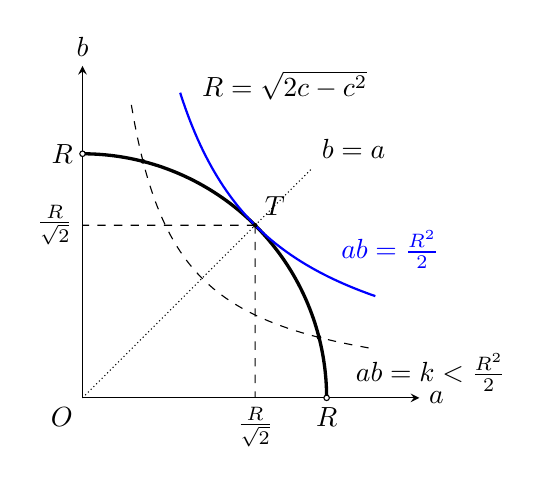
\begin{tikzpicture}[scale=3.1,>=stealth]
      % R=\sqrt{2c-c^2} で規格化した第1象限の円弧．
      \draw[->] (0,0) -- (1.38,0) node[right] {$a$};
      \draw[->] (0,0) -- (0,1.36) node[above] {$b$};
      \node[below left] at (0,0) {$O$};
      \draw[very thick,domain=0:90,samples=81]
      plot ({cos(\x)},{sin(\x)});
      \draw[dashed,domain=0.20:1.2,samples=81]
      plot (\x,{0.24/\x});
      \draw[blue,thick,domain=0.40:1.2,samples=81]
      plot (\x,{0.5/\x});
      \draw[densely dotted] (0,0) -- (0.94,0.94) node[above right] {$b=a$};
      \coordinate (T) at ({sqrt(0.5)},{sqrt(0.5)});
      \draw[dashed] (T) -- ({sqrt(0.5)},0);
      \draw[dashed] (T) -- (0,{sqrt(0.5)});
      \node[circle, fill, inner sep=0.6pt] at (T) {}; \node[above right] at (T) {$T$};
      \node[circle, fill, inner sep=0.6pt] at ({sqrt(0.5+sqrt(0.25-0.24^2))},{sqrt(0.5-sqrt(0.25-0.24^2))}) {};
      \node[circle, fill, inner sep=0.6pt] at ({sqrt(0.5-sqrt(0.25-0.24^2))},{sqrt(0.5+sqrt(0.25-0.24^2))}) {};
      \node[circle, draw, fill=white, inner sep=0.7pt] at (1,0) {};
      \node[circle, draw, fill=white, inner sep=0.7pt] at (0,1) {};
      \node[below] at (1,0) {$R$};
      \node[left] at (0,1) {$R$};
      \node[below] at ({sqrt(0.5)},0) {$\frac{R}{\sqrt{2}}$};
      \node[left] at (0,{sqrt(0.5)}) {$\frac{R}{\sqrt{2}}$};
      \node[below right] at (1.08,{0.24/1.08}) {$ab=k<\frac{R^2}{2}$};
      \node[above right,blue] at (1.02,{0.5/1.02}) {$ab=\frac{R^2}{2}$};
      \node[above right] at (0.45,1.18) {$R=\sqrt{2c-c^2}$};
    \end{tikzpicture}
  \end{center}
  \caption{$c$を固定したときの円弧（太線）と双曲線$ab=k$．$T$で接するとき$ab$が最大となる．}
  \label{fig:utokyo1987q3_circle_hyperbola}
\end{figure}

従ってこれと$k=ab$の交点を考えて，$ab$は$(a,b)=\left(\sqrt{\dfrac{2c-c^2}{2}},\sqrt{\dfrac{2c-c^2}{2}}\right)$で最大値$\max ab = \dfrac{2c-c^2}{2}$をとる．
従って$c$を固定した時の面積$S$の最小値は\cref{eq:4}から
\begin{align}
  \min S
  &= \dfrac{1}{2c-c^2}\dfrac{c^2}{c-1} \\
  &=\dfrac{1}{3-(c+2/c)}
\end{align}
である．次に$c$を$1<c<2$の範囲で動かすと，$y=c+\dfrac{2}{c}$は以下のようになる．

\begin{figure}[htbp]
  \begin{center}
    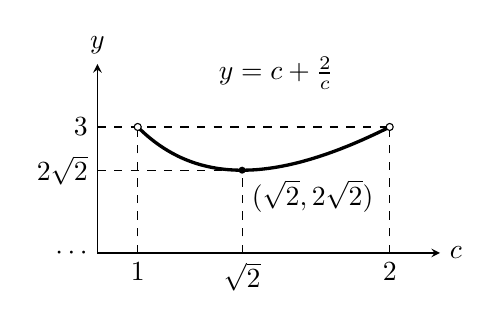
\begin{tikzpicture}[xscale=3.2,yscale=3.2,>=stealth]
      % y方向は2.5だけ平行移動して表示．
      \draw[->] (0.84,0) -- (2.20,0) node[right] {$c$};
      \draw[->] (0.84,0) -- (0.84,0.75) node[above] {$y$};
      \draw[dashed] (0.84,0.5) -- (2,0.5);
      \draw[dashed] (1,0) -- (1,0.5);
      \draw[dashed] (2,0) -- (2,0.5);
      \draw[dashed] ({sqrt(2)},0) -- ({sqrt(2)},{2*sqrt(2)-2.5});
      \draw[dashed] (0.84,{2*sqrt(2)-2.5}) -- ({sqrt(2)},{2*sqrt(2)-2.5});
      \draw[very thick,domain=1:2,samples=101] plot (\x,{\x+2/\x-2.5});
      \node[circle, draw, fill=white, inner sep=0.9pt] at (1,0.5) {};
      \node[circle, draw, fill=white, inner sep=0.9pt] at (2,0.5) {};
      \node[circle, fill, inner sep=0.9pt] at ({sqrt(2)},{2*sqrt(2)-2.5}) {};
      \node[below] at (1,0) {$1$};
      \node[below] at ({sqrt(2)},0) {$\sqrt{2}$};
      \node[below] at (2,0) {$2$};
      \node[left] at (0.84,0.5) {$3$};
      \node[left] at (0.84,{2*sqrt(2)-2.5}) {$2\sqrt{2}$};
      \node[above] at (1.55,0.61) {$y=c+\frac{2}{c}$};
      \node[below right] at ({sqrt(2)},{2*sqrt(2)-2.5}) {$(\sqrt{2},2\sqrt{2})$};
      \node[left] at (0.84,0) {$\cdots$};
    \end{tikzpicture}
  \end{center}
  \caption{$1<c<2$における$y=c+\dfrac{2}{c}$のグラフ．両端の白丸は範囲に含まない．}
  \label{fig:utokyo1987q3_c_function}
\end{figure}

従って$2\sqrt{2}\le y$だから，$c$を動かした時の$S$の最小値は
\begin{align}
  \min S = \dfrac{1}{3-2\sqrt{2}} = 3+2\sqrt{2}
\end{align}
である．

\newpage
\end{document}
